\documentclass[14pt]{extarticle}
\usepackage{fontspec}
\usepackage{geometry}
\geometry{a4paper, margin=2.2cm}
\usepackage{graphicx}
\usepackage{booktabs}
\usepackage{array}
\usepackage{caption}
\usepackage{enumitem}
\usepackage{amsmath}
\usepackage[table]{xcolor}
\usepackage{titlesec}
\usepackage{fancyhdr}

% ---- Thai font (THSarabunNew) ----
\setmainfont{THSarabunNew.ttf}[
  Path=./fonts/,
  BoldFont=THSarabunNew Bold.ttf,
  ItalicFont=THSarabunNew Italic.ttf,
  BoldItalicFont=THSarabunNew BoldItalic.ttf]
\XeTeXlinebreaklocale "th"
\XeTeXlinebreakskip = 0pt plus 0.1pt

\definecolor{brand}{HTML}{c1121f}
\definecolor{ink}{HTML}{1c2330}
\titleformat{\section}{\Large\bfseries\color{brand}}{\thesection.}{0.5em}{}
\titleformat{\subsection}{\large\bfseries\color{ink}}{\thesubsection}{0.5em}{}
\captionsetup{font=small, labelfont={bf,color=brand}}
\setlist{itemsep=1pt, topsep=3pt}
\pagestyle{fancy}\fancyhf{}
\fancyhead[L]{\small\color{ink} X-ray Pelvis SPR — Fracture Detection}
\fancyhead[R]{\small\color{ink}\thepage}
\renewcommand{\headrulewidth}{0.4pt}

\begin{document}

\begin{center}
{\LARGE\bfseries\color{brand} รายงานผลการดำเนินงานและวิเคราะห์เบื้องต้น}\\[4pt]
{\Large การตรวจจับรอยแตกกระดูกเชิงกรานด้วยลายเซ็นการกระเจิงรังสีเอกซ์}\\
{\large (Scatter-to-Primary Ratio Signature) จากการจำลอง Monte Carlo}\\[8pt]
{\small ระบบจำลอง OpenGATE 10 / Geant4 \quad$\bullet$\quad รายงานฉบับเบื้องต้นประกอบข้อเสนอโครงการ}\\
{\small \today}
\end{center}
\vspace{4pt}
\hrule
\vspace{10pt}

\section*{บทคัดย่อ}
โครงการนี้ศึกษาความเป็นไปได้ในการตรวจจับ ``รอยแตกกระดูก'' ขนาดเล็กระดับต่ำกว่ามิลลิเมตร
จากภาพรังสีเอกซ์ โดยอาศัย \textbf{ลายเซ็นการกระเจิงรังสี} ที่วัดผ่านอัตราส่วนการกระเจิงต่อรังสีปฐมภูมิ
(Scatter-to-Primary Ratio, SPR) ด้วยการจำลองแบบ Monte Carlo (OpenGATE~10 / Geant4)
รายงานฉบับนี้นำเสนอ (1)~ระเบียบวิธีที่พัฒนาขึ้นเพื่อแยกสัญญาณของรอยแตกออกจากสัญญาณรบกวนอย่างถูกต้อง
ได้แก่ การออกแบบกลุ่มควบคุมที่ใช้ฐานเรขาคณิตเดียวกัน (\textit{matched control}) และการวิเคราะห์นัยสำคัญ
เชิงสถิติแบบหลายเมล็ดสุ่ม (\textit{multi-seed significance}) และ (2)~ผลเบื้องต้นซึ่งแสดงว่าสัญญาณ SPR
จากรอยแตกสามารถ\textbf{ตรวจพบได้อย่างมีนัยสำคัญที่รอยแตกทั้งสี่ขนาด} (0.306--1.0~มม.; ทุกขนาด $p<0.02$)
โดย\textbf{ความแรงของสัญญาณเพิ่มขึ้นตามขนาดรอยแตกในช่วง 0.306--0.54~มม.} แล้วเข้าสู่ระดับอิ่มตัว
ในขณะที่บริเวณอ้างอิงไม่มีนัยสำคัญ (null) ทุกกรณี ซึ่งสนับสนุนว่าสัญญาณที่วัดได้มีต้นกำเนิดจากรอยแตกจริง
มิใช่สัญญาณรบกวน นอกจากนี้ยังพบว่า\textbf{ระดับ SPR เอง}เป็นตัวชี้วัดที่จับสัญญาณได้ ในขณะที่ตัวชี้วัดเชิง
พื้นผิว (local variance, entropy) ไม่ไวต่อสัญญาณนี้

\section{บทนำและวัตถุประสงค์}
รอยแตกกระดูกแบบเส้นผม (hairline / sub-millimetre fracture) มักตรวจพบได้ยากในภาพรังสีทั่วไป
เนื่องจากความแตกต่างของการดูดกลืนรังสี (attenuation) ที่รอยแตกสร้างขึ้นมีค่าน้อยมาก
สมมติฐานหลักของโครงการคือ รอยแตกทำให้เกิดการเปลี่ยนแปลงเฉพาะจุดของ\textbf{องค์ประกอบการกระเจิงรังสี}
ซึ่งอาจให้ ``ลายเซ็น'' ที่ตรวจจับได้ดีกว่าการดูกลืนโดยตรง

\noindent\textbf{วัตถุประสงค์ของงานในระยะนี้:}
\begin{itemize}
  \item สร้างแบบจำลอง Monte Carlo ที่แยกรังสีปฐมภูมิ (primary) ออกจากรังสีกระเจิง (scatter)
        ณ ระนาบฉากรับ เพื่อคำนวณแผนที่ SPR
  \item พัฒนาระเบียบวิธีวิเคราะห์ที่\textbf{แยกสัญญาณของรอยแตกออกจากปัจจัยรบกวน}ได้อย่างถูกต้อง
  \item ทดสอบว่าสัญญาณ SPR จากรอยแตกตรวจพบได้อย่างมีนัยสำคัญเชิงสถิติหรือไม่ และหา
        \textbf{ขีดจำกัดการตรวจจับ (detectability threshold)} ตามขนาดรอยแตก
\end{itemize}

\section{ระเบียบวิธี}

\subsection{การจำลองด้วย Monte Carlo}
ใช้ OpenGATE~10 (Geant4) จำลองภาพรังสีเชิงกรานแบบ AP โดยมีพารามิเตอร์มาตรฐานดังตาราง~\ref{tab:sim}
แบบจำลองแยกโฟตอนที่ระนาบฉากรับออกเป็นปฐมภูมิ/กระเจิง โดยพิจารณาจากมุมเบี่ยงเบนจากแนวรังสีตรง
($\le 0.5^\circ$) ร่วมกับความเบี่ยงเบนพลังงาน ($|E-E_0|\le 1$~keV) แล้วคำนวณ
$\mathrm{SPR}=I_{\text{scatter}}/I_{\text{primary}}$ เป็นภาพเชิงพื้นที่

\begin{table}[h]\centering
\caption{พารามิเตอร์การจำลองมาตรฐาน}\label{tab:sim}
\small
\begin{tabular}{ll}
\toprule
\textbf{พารามิเตอร์} & \textbf{ค่า} \\
\midrule
Engine / Physics list & OpenGATE 10 (Geant4), \texttt{G4EmLivermorePhysics} \\
แหล่งกำเนิด & แกมมา point source, 80~keV mono \\
วัสดุวัตถุ & \texttt{G4\_BONE\_COMPACT\_ICRU} \\
เรขาคณิต & SOD 800~มม., ODD ปรับได้, ฉากรับตั้งฉากแนวลำแสง \\
แบบจำลองรอยแตก & pelvis STL, ช่องว่างรอยแตก 0.306 / 0.43 / 0.54 / 1.0~มม. \\
\bottomrule
\end{tabular}
\end{table}

\subsection{การออกแบบกลุ่มควบคุมฐานเดียวกัน (Matched Control) --- จุดสำคัญเชิงระเบียบวิธี}
การวิเคราะห์เบื้องต้นพบว่า การนำแบบจำลอง ``ปกติ'' (control) กับ ``รอยแตก'' (fracture) ที่เป็น
\textbf{คนละ mesh กัน}มาเปรียบเทียบ ทำให้ผลต่าง $\Delta\mathrm{SPR}$ ถูกครอบงำด้วยความแตกต่างของ
เรขาคณิต/การแบ่ง mesh ทั้งก้อน มิใช่รอยแตก (สัญญาณคงที่ทุกขนาด ไม่ขึ้นกับความกว้างรอยแตก)
ซึ่งเป็นเหตุให้ผลก่อนหน้ายัง \textit{inconclusive}

เพื่อขจัดปัจจัยรบกวนนี้ ผู้วิจัยสร้างกลุ่มควบคุมจาก\textbf{ฐาน mesh เดียวกันกับรอยแตก}
โดย ``ถม'' ร่องรอยแตกด้วยกระดูก (boolean union กับกล่องบางที่วางตามระนาบรอยแตก)
ผลลัพธ์ผ่านการตรวจสอบว่า control กับ fracture มีผิวตรงกันทุกจุด\textbf{นอกบริเวณรอยแตก}
(ความคลาดเคลื่อน 0.0000~มม. จากจุดยอดกว่า 349{,}000 จุด) ทำให้ผลต่าง
$\Delta\mathrm{SPR}=\mathrm{SPR}_{\text{fracture}}-\mathrm{SPR}_{\text{control}}$
\textbf{แยกเฉพาะผลของรอยแตกล้วน ๆ}

\subsection{การวิเคราะห์นัยสำคัญแบบหลายเมล็ดสุ่ม (Multi-Seed Significance)}
การจำลอง Monte Carlo แต่ละครั้งให้ผลเพียงหนึ่งการรับรู้ (realization) จึงแยกไม่ได้ว่าสัญญาณจริง
หรือเป็นสัญญาณรบกวน ผู้วิจัยรันกระบวนการทั้งหมดซ้ำด้วยเมล็ดสุ่ม (random seed) อิสระ $N=8$ ชุด
(ภายในแต่ละชุด control และ fracture ใช้เมล็ดเดียวกัน = \textit{common random numbers} เพื่อลดความแปรปรวน
ของผลต่าง) แล้วคำนวณ\textbf{แผนที่นัยสำคัญต่อพิกเซล} ($t=\text{mean}/(\text{s.d.}/\sqrt{N})$)
พร้อมสถิติ $t$ และ $p$-value ในบริเวณสนใจ (ROI) ที่ตำแหน่งรอยแตก ซึ่งกำหนดไว้ล่วงหน้า
(\textit{a-priori}) เทียบกับบริเวณอ้างอิง (background)

\subsection{การบีบลำแสงและระบบคำนวณ}
บีบลำแสง (collimation) ให้จ่อเฉพาะบริเวณรอยแตก เพื่อเพิ่มจำนวนโฟตอนต่อพิกเซล
(ในการทดลองนี้ $\sim$3{,}600 โฟตอน/พิกเซล) การคำนวณดำเนินบนระบบที่พัฒนาขึ้นซึ่งกระจายงานแบบ
multi-process (sharding) และรองรับการสั่งงานทางไกลผ่านเซิร์ฟเวอร์ ทำให้ทำ parameter sweep
ได้อย่างเป็นระบบและทำซ้ำได้

\section{ผลการดำเนินงานเบื้องต้น}

\subsection{ความจำเป็นของ Matched Control}
เมื่อใช้กลุ่มควบคุมคนละ mesh ค่า $\Delta\mathrm{SPR}$ เฉลี่ยเกือบคงที่ทุกขนาดรอยแตก
(เช่น $\sim -0.007$ ที่สนามเต็ม) และไม่แปรตามความกว้างรอยแตก บ่งชี้ว่าเป็นผลของความต่างของ mesh
มิใช่รอยแตก เมื่อเปลี่ยนมาใช้ matched control สัญญาณที่แท้จริงจึงปรากฏ

\subsection{การตรวจพบสัญญาณและแนวโน้มตามขนาดรอยแตก}
ตาราง~\ref{tab:res} สรุปผลที่บริเวณรอยแตก (ROI 16$\times$16 พิกเซล กำหนดล่วงหน้าที่ตำแหน่งลำแสงจ่อ)
เทียบกับบริเวณอ้างอิง จะเห็นว่าสัญญาณที่รอยแตก\textbf{มีนัยสำคัญครบทั้งสี่ขนาด} ($p<0.02$ ทุกกรณี)
โดย\textbf{ความแรง ($|t|$) เพิ่มขึ้นตามขนาดรอยแตก}ในช่วง 0.306--0.54~มม. ($|t|=3.12\to3.66\to4.84$)
แล้วเข้าสู่ระดับอิ่มตัว (1.0~มม. ให้ $|t|=4.32$ ซึ่งเทียบเท่า 0.54~มม. ในเชิงสถิติ) ในขณะที่บริเวณอ้างอิง
\textbf{ไม่มีนัยสำคัญ (null) ทุกกรณี} --- ยืนยันความจำเพาะเชิงพื้นที่ของสัญญาณ

\begin{table}[h]\centering
\caption{ผลนัยสำคัญที่บริเวณรอยแตก (matched control, $N=8$ เมล็ดสุ่ม)}\label{tab:res}
\small
\begin{tabular}{c c c c c}
\toprule
\textbf{ขนาดรอยแตก} & \textbf{$\Delta$SPR (ROI)} & \textbf{$t$} & \textbf{$p$-value} & \textbf{background ($p$)} \\
\midrule
0.306 มม. & $-3.3\times10^{-5}$ & $-3.12$ & \textbf{0.017} & 0.93 (null) \\
0.43 มม.\  & $-3.4\times10^{-5}$ & $-3.66$ & \textbf{0.008} & 0.47 (null) \\
0.54 มม.\  & $-4.9\times10^{-5}$ & $-4.84$ & \textbf{0.002} & 0.57 (null) \\
1.0 มม.\   & $-4.2\times10^{-5}$ & $-4.32$ & \textbf{0.004} & 0.30 (null) \\
\bottomrule
\end{tabular}
\end{table}

เครื่องหมายลบของ $\Delta\mathrm{SPR}$ สอดคล้องกับหลักฟิสิกส์: ที่รอยแตก (ช่องว่างอากาศ)
รังสีปฐมภูมิทะลุผ่านมากขึ้น ทำให้อัตราส่วน scatter/primary ลดลงเฉพาะจุด

\begin{figure}[h]\centering
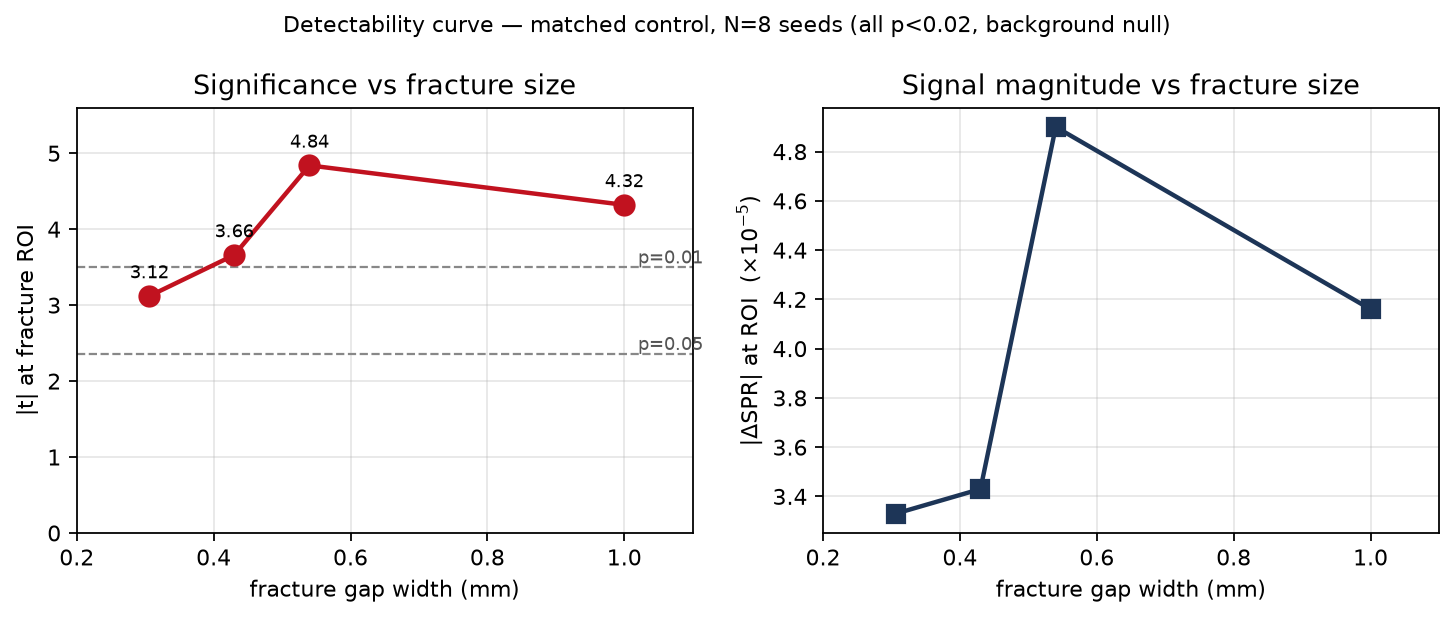
\includegraphics[width=0.98\textwidth]{fig/trend.png}
\caption{เส้นโค้ง detectability ครบทั้งสี่ขนาด. \textbf{ซ้าย:} ความแรงของสัญญาณ ($|t|$) ที่บริเวณรอยแตก
เพิ่มขึ้นตามขนาดในช่วง 0.306--0.54~มม. แล้วเข้าสู่ระดับอิ่มตัว (เส้นประ = ระดับนัยสำคัญ $p=0.05$ และ $p=0.01$).
\textbf{ขวา:} ขนาดสัญญาณ $|\Delta\mathrm{SPR}|$ ให้รูปแบบเดียวกัน; ทุกขนาดมีนัยสำคัญ ($p<0.02$) และ background เป็น null}
\label{fig:trend}
\end{figure}

\begin{figure}[h]\centering
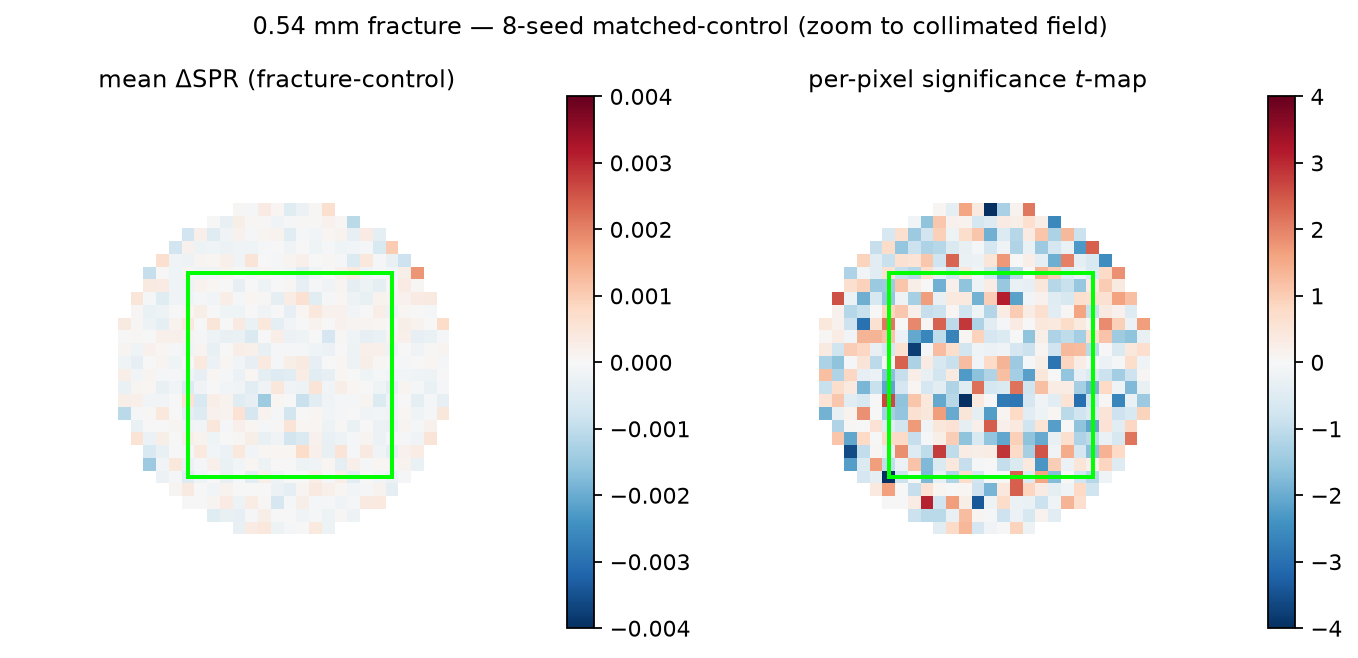
\includegraphics[width=0.92\textwidth]{fig/sigmap.png}
\caption{แผนที่ผลต่าง SPR เฉลี่ย (ซ้าย) และแผนที่นัยสำคัญ $t$ ต่อพิกเซล (ขวา) ของรอยแตก 0.54~มม.
(ขนาดที่ให้สัญญาณแรงสุด) กรอบสีเขียวคือ ROI ที่กำหนดล่วงหน้าที่ตำแหน่งรอยแตก}
\label{fig:sig}
\end{figure}

\section{อภิปราย}
ผลเบื้องต้นให้ข้อสรุปเชิงระเบียบวิธีและเชิงฟิสิกส์ที่สำคัญสองประการ:
\begin{enumerate}
  \item \textbf{ระเบียบวิธีเป็นตัวชี้ขาด:} การเปรียบเทียบแบบไร้เดียงสา (control คนละ mesh, เมล็ดเดียว)
        ให้ผล null/inconclusive เพราะสัญญาณรอยแตกถูกกลบด้วยความต่างของ mesh และสัญญาณรบกวน
        เมื่อควบคุมทั้งสองปัจจัย (matched control + multi-seed) สัญญาณที่แท้จริงจึงปรากฏ
  \item \textbf{มีหลักฐานสนับสนุนสัญญาณจริง:} สัญญาณมีนัยสำคัญที่ตำแหน่งรอยแตกซึ่งกำหนดไว้ล่วงหน้า
        (ทั้งสี่ขนาด $p<0.02$) ในขณะที่บริเวณอ้างอิงเป็น null และ\textbf{ความแรงเพิ่มขึ้นตามขนาดรอยแตก}
        (dose--response) ในช่วง 0.306--0.54~มม. ก่อนเข้าสู่ระดับอิ่มตัว ซึ่งเป็นรูปแบบที่คาดหวังของสัญญาณ
        เชิงสาเหตุ มิใช่สัญญาณรบกวนแบบสุ่ม (การอิ่มตัวที่ขนาดใหญ่ยังต้องตรวจสอบ---อาจเกิดจาก ROI ขนาดคงที่
        หรือขีดจำกัดสถิติที่ $N=8$)
  \item \textbf{ระดับ SPR คือตัวชี้วัดที่ถูกต้อง:} เมื่อทดสอบตัวชี้วัดเชิงพื้นผิว (local variance และ local
        entropy บนแผนที่ SPR) พบว่า\textbf{ไม่ไวต่อสัญญาณ}เลย (ทุกขนาด $p>0.25$) เพราะรอยแตกทำให้ระดับ SPR
        เลื่อนลงอย่างเรียบและสม่ำเสมอ (mean shift) ซึ่งตัวชี้วัดความแปรปรวนไม่รับรู้โดยธรรมชาติ
        ($\mathrm{STD}(x+c)=\mathrm{STD}(x)$) --- ผลนี้ชี้ชัดว่าลายเซ็นอยู่ที่\textbf{ระดับ SPR เอง}
\end{enumerate}

\section{ข้อจำกัดและงานถัดไป}
\begin{itemize}
  \item ผลปัจจุบันครอบคลุม\textbf{ครบทั้งสี่ขนาด} ($N=8$ เมล็ด) แต่ยังเป็น\textbf{เบื้องต้น} ---
        สัญญาณที่รอยแตกเล็กสุด (0.306~มม.) ยัง\textbf{ก้ำกึ่ง} และเส้นโค้งเข้าสู่ระดับอิ่มตัวที่ขนาดใหญ่
        ควรเพิ่มจำนวนเมล็ด/สถิติเพื่อยืนยันและระบุสาเหตุการอิ่มตัว รวมถึงพิจารณาการแก้ไข multiple comparison
  \item ตรวจสอบผลการอิ่มตัว (1.0~มม. ไม่สูงกว่า 0.54~มม.) ด้วย ROI ที่ปรับตามขนาดรอยแตก
        และสถิติที่สูงขึ้น เพื่อยืนยันเส้นโค้ง detectability threshold
  \item ขยายการศึกษาไปยังตำแหน่ง/ทิศทางรอยแตกอื่น, พลังงานลำแสงอื่น, และแบบจำลองฉากรับเชิงจริง
        (ประสิทธิภาพเชิงพลังงาน, จุดกระเจิงในฉากรับ) รวมถึงการเทียบกับข้อมูลภาพจริง
\end{itemize}

\section{สรุป}
งานในระยะนี้ได้พัฒนา\textbf{ระเบียบวิธีที่ถูกต้อง}สำหรับตรวจวัดลายเซ็นการกระเจิงจากรอยแตก
(matched control เพื่อตัด confound และ multi-seed significance เพื่อวัดนัยสำคัญ)
และแสดง\textbf{หลักฐานเชิงประจักษ์เบื้องต้น}ว่าสัญญาณ SPR จากรอยแตกขนาดต่ำกว่ามิลลิเมตร
สามารถตรวจพบได้อย่างมีนัยสำคัญและแปรตามขนาดรอยแตก ผลนี้เป็น \textit{proof-of-concept}
ที่สนับสนุนความเป็นไปได้ของแนวทาง และเป็นฐานสำหรับการศึกษาเชิงปริมาณที่สมบูรณ์ในโครงการต่อไป

\vfill
\noindent\rule{\textwidth}{0.4pt}\\
{\small\color{ink} จัดทำจากผลการดำเนินงานจริงของระบบจำลอง (repository: \texttt{GATE-Xray-pelvis-SPR}).
รูปและตัวเลขทั้งหมดคำนวณจากผลการรันจริง.}

\end{document}
